\section{Experiments}
\begin{table}[!t]
\centering
\caption{Acceptance length $\tau$ evaluation on general-purpose workloads.}
\label{tab:acceptance_length}
\small
\setlength{\tabcolsep}{4.2pt} % <--- 增加一列后内容变宽，适当调小列间距
\renewcommand{\arraystretch}{1.1}
\begin{tabular}{llccccccc} % <--- 恢复为9列 (2l + 7c)
\toprule
& & \multicolumn{2}{c}{\textbf{Math}} & \multicolumn{3}{c}{\textbf{Code}} & \multicolumn{2}{c}{\textbf{Chat}} \\ % <--- Code改为跨3列
\cmidrule(lr){3-4} \cmidrule(lr){5-7} \cmidrule(lr){8-9}          % <--- cmidrule范围改为5-7
\textbf{Model} & \textbf{Method} & \textbf{GSM8K} & \textbf{MATH-500} & \textbf{HumanEval} & \textbf{\ MBPP} & \textbf{\ \ \ LCB \ \ } & \textbf{MT-Bench} & \textbf{Alpaca} \\
\midrule
\multirow{6}{*}{Qwen3-4B}   & EAGLE3 & 2.63 & 2.39 & 2.47 & 2.34 & 2.17 & 3.07 & 2.28 \\
                            & DFlow  & 5.13 & 4.92 & 4.33 & 4.12 & - & 3.80 & 2.90 \\
                            & DFlash    & 5.97 & 5.82 & 5.25 & 4.97 & 4.82 & 3.39 & 3.56 \\
                            & DFlash2    & 6.14 & 5.80 & 5.38 & 5.14 & 4.79 & \textbf{4.14} & 2.50 \\
                            & DSpark    & 6.27 & 6.25 & 5.62 & 5.48 & 5.20  & 3.81 & 3.54 \\
                            & DLite     & \textbf{6.38} & \textbf{6.30} & \textbf{5.68} & \textbf{5.64} & \textbf{5.31} & 3.94 & \textbf{3.64} \\
\midrule
\multirow{5}{*}{Qwen3-8B}   & EAGLE3 & 2.60 & 2.28 & 2.51 & 2.17 & 2.08 & 3.07 & 2.56 \\
                            & DFlow  & 5.10 & 4.94 & 4.28 & 4.08 & - & 3.58 & 2.93 \\
                            & DFlash    & 6.04 & 5.91 & 5.27 & 4.88 & 4.89 & 3.39 & 3.56 \\
                            & DSpark    & 6.36 & 6.34 & 5.86 & 5.36 & 5.43 & 3.88 & 3.64 \\
                            & DLite     & \textbf{6.48} & \textbf{6.35} & \textbf{5.96} & \textbf{5.65} & \textbf{5.66} & \textbf{3.96} & \textbf{3.78} \\
\bottomrule
\end{tabular}
\end{table}



\subsection{Experimental Setup} \label{sec:exp:setup}

% \textbf{Models and Evaluations.} We conduct experiments on Qwen3-4B, Qwen3-8B and Qwen3.5-4B models. We compare \we with vanilla autoregressive decoding (baseline) and open-sourced state-of-the-art speculative decoding method EAGLE-3~\cite{li2026eagle3}, DFlash~\cite{chen2026dflash}, DFlash2~\cite{dflash2}, DSpark~\cite{cheng2026dspark}, DFlow~\cite{zhang2026dflow}. We evaluate the performance in two different domains, general-purpose tasks and agentic tasks. General-purpose tasks include four categories, Math: GSM8K and MATH-500, Code: HumanEval, MBPP, and LiveCodeBench (LCB), Chat: MT-Bench and Alpaca, LongBench v2: Multi-Document QA (Multi-Doc QA), Long In-context Learning (Long In-ctx Lrn), Code Repository Understanding (Code Repo Ud), and Long dialogue History (Long-dialog Hist). Agentic tasks include AgentMemoryBench, AgentLongBench, BFCL-v3, SWE-Bench. We conduct all experiments on NVIDIA H800 GPUs.


\textbf{Models and Baselines.} We evaluate \we on Qwen3-4B and Qwen3-8B. We compare against vanilla autoregressive decoding (baseline) and representative speculative decoding methods, including EAGLE-3~\cite{li2026eagle3}, DFlash~\cite{chen2026dflash}, DFlash2~\cite{dflash2}, DSpark~\cite{cheng2026dspark}, and DFlow~\cite{zhang2026dflow}. All serving experiments are conducted on NVIDIA H800 GPUs. The results of DFlash2 and DFlow are from RedHatAI~\cite{redhat} or paper.

% \textbf{Benchmarks.} We evaluate the performance in three different domains, general-purpose tasks, long-context tasks and agentic tasks. General-purpose tasks include three categories, Math: GSM8K and MATH-500, Code: HumanEval, MBPP, and LiveCodeBench (LCB), Chat: MT-Bench and Alpaca. Long-context taskss include Multi-Document QA (Multi-Doc QA), Long In-context Learning (Long In-ctx Lrn), Code Repository Understanding (Code Repo Ud), and Long dialogue History (Long-dialog Hist). Agentic tasks include AgentMemoryBench, AgentLongBench, BFCL-v3, SWE-Bench.

\textbf{Benchmarks.} We evaluate the performance in three different domains, general-purpose tasks, long-context tasks and agentic tasks. General-purpose tasks include three categories, Math: GSM8K~\cite{gsm8k} and MATH-500~\cite{math500}, Code: HumanEval~\cite{humaneval}, MBPP~\cite{MBPP}, and LiveCodeBench~\cite{jain2025livecodebench}, Chat: MT-Bench~\cite{zheng2023judging} and Alpaca~\cite{alpaca}. Long-context tasks include Multi-Document QA, Long In-context Learning, Code Repository Understanding, and Long dialogue History in LongBench\_v2~\cite{bai2024longbench}. Agentic tasks include AgentMemoryBench~\cite{liu2024agentbench}, AgentLongBench~\cite{fang2026agentlongbenchcontrollablelongbenchmark}, BFCL-v3~\cite{bfcl} and SWE-Bench~\cite{jimenez2024swebench}.


\textbf{Datasets.}
We use Open-PerfectBlend~\cite{xu2024perfect} which consists of 1.3 million samples containing chat, math, code and instruction-following data. We also collect 600K samples from NVIDIA Nemotron Post-Training Dataset V2~\cite{NemotronPostTrainingDatasetV2} to augment the dataset. We only use the prompts from the dataset and generate the response using the target models.

\textbf{Implementation Details.} For all speculative decoding methods, we use a speculative block size of \(K=7\) and follow the original implementation whenever available. \we uses 12/14 layer target hidden states with sequence-wise concatenation, and a sequential-head rank of \(R=320/512\) for Qwen3-4B/8B. We report average acceptance length \(\tau\) and end-to-end decoding speedup over vanilla autoregressive decoding. 
% For high-concurrency experiments, we additionally report aggregate throughput in tokens per second (TPS) under concurrency levels \(1,8,16,32,\) and \(64\). Additional training and serving configurations are provided in Appendix [X].





\subsection{Performance Evaluation}


\textbf{General-purpose workloads.} Table~\ref{tab:acceptance_length}  reports acceptance lengths on conventional reasoning, coding, and conversational benchmarks. \we consistently matches or outperforms existing speculative drafters on both Qwen3-4B and Qwen3-8B. These results show that removing the historical draft KV cache does not sacrifice drafting quality on standard workloads, despite \we operating only on target representations and a local anchor token. 


% Table~\ref{tab:acceptance_length} reports the average acceptance length on conventional reasoning, coding, and conversational benchmarks. \we consistently matches or outperforms existing speculative drafters across both Qwen3-4B and Qwen3-8B. In particular, \we achieves acceptance lengths of 6.38/6.48 on GSM8K, 5.64/5.65 on MBPP, and 5.31/5.66 on LiveCodeBench for the 4B/8B models, respectively. It also consistently improves over the strongest semi-autoregressive baseline, DSpark, across all reported benchmarks. These results indicate that removing the historical draft KV cache does not sacrifice drafting quality on conventional workloads. Although \we only operates on compact target representations and a fixed local window, these inputs retain sufficient contextual information for accurate speculation. The improvement is moderate on these relatively standard workloads, where existing drafters already achieve high acceptance lengths; as shown next, the difference becomes substantially larger as contextual modeling becomes more challenging.

%  ------------------------------
\textbf{Long-context workloads.} 
As shown in Table~\ref{tab:longbench_v2_models}, the advantage of \we becomes more pronounced on LongBench v2, where it consistently improves both acceptance length and end-to-end speedup over DFlash and DSpark. This trend supports our central design motivation: as the context grows, conventional drafters increasingly rely on their own long-history modeling, whereas \we delegates global-context modeling to the target model and performs only local prediction at the draft side.
% The advantage of \we becomes more pronounced on long-context workloads. As shown in Table~\ref{tab:longbench_v2_models}, \we consistently improves both acceptance length and end-to-end speedup across all four LongBench v2 categories. On Qwen3-4B, DLite achieves speedups of $1.66\sim2.86\times$, compared with 1.31\(\sim\)2.45\(\times\) for DSpark. The improvement is particularly clear on Code Repository Understanding, where \we increases the speedup from 1.39\(\times\) to 1.93\(\times\) while increasing the acceptance length from 2.35 to 3.14.

% More importantly, the relative advantage over conventional drafters increases compared with the general-purpose benchmarks. This observation is consistent with the motivation of DLite: as the accumulated context becomes longer, conventional lightweight drafters must increasingly reconstruct long-range contextual information using their own historical states, whereas DLite delegates this task to the target model and keeps the draft-side prediction problem fixed in size. Consequently, its drafting quality degrades less severely as context complexity increases.
\textbf{Agentic workloads.} 
Table~\ref{tab:agent_benchmarks} shows the largest relative gains under agentic workloads. In particular, on SWE-Bench, \we substantially improves acceptance length over DFlash and DSpark while achieving around \(2\times\) end-to-end speedup. These results indicate that history-free drafting is especially beneficial under the long, evolving contexts characteristic of agent execution


% ---------------- longbench ------------------
\begin{table}[!t]
\centering
\vspace{-10pt}
\caption{Speedup and acceptance length ($\tau$) evaluation on long-context workloads.}
\label{tab:longbench_v2_models}
\small
\renewcommand{\arraystretch}{1.1}
\setlength{\tabcolsep}{5.8pt} % 列较多，适当减小间距
\begin{tabular}{c l cc cc cc cc}
\toprule
\multirow{3}{*}{\textbf{Model}} & \multirow{3}{*}{\textbf{Method}} & \multicolumn{8}{c}{\textbf{LongBench\_v2}} \\
\cmidrule(lr){3-10}
& & \multicolumn{2}{c}{\textbf{Multi-Doc QA}} & \multicolumn{2}{c}{\textbf{Long In-ctx Lrn.}} & \multicolumn{2}{c}{\textbf{Code Repo Ud.}} & \multicolumn{2}{c}{\textbf{Long-dialog Hist.}} \\
\cmidrule(lr){3-4} \cmidrule(lr){5-6} \cmidrule(lr){7-8} \cmidrule(lr){9-10}
& & Speedup & $\tau$ & Speedup & $\tau$ & Speedup & $\tau$ & Speedup & $\tau$ \\
\midrule

% --- Qwen3-4B Data (From Image 1) ---
\multirow{4}{*}{Qwen3-4B} 
& Eagle3      & 1.70$\times$ & 2.10  & 1.76$\times$  & 2.28   & 1.68$\times$  & 2.12 & 2.23$\times$  & 2.88   \\
& DFlash     & 1.60$\times$  & 1.90 & 1.71$\times$ & 2.00 & 1.45$\times$ & 1.83 & 2.62$\times$ & 3.04 \\
& DSpark     & 1.81$\times$ & 2.20 & 2.01$\times$ & 2.41 & 2.02$\times$ & 2.44 & 3.16$\times$ & 3.93 \\
& DLite & \textbf{2.18$\times$} & \textbf{2.74} & \textbf{2.58$\times$} & \textbf{3.11} & \textbf{2.66$\times$} & \textbf{3.14} & \textbf{3.88$\times$} & \textbf{4.62} \\

\midrule

% --- Qwen3-8B Data (From Image 2) ---
\multirow{4}{*}{Qwen3-8B}
& Eagle3      & 1.64$\times$ & 2.05 & 1.87$\times$ & 2.33 & 1.42$\times$  & 1.80 & 2.01$\times$  & 2.56 \\
& DFlash     & 1.81$\times$  & 2.10 & 1.86$\times$ & 2.28 & 1.65$\times$  & 2.16 & 2.58$\times$  & 3.07 \\
& DSpark     & 1.98$\times$  & 2.52 & 2.28$\times$ & 2.67 & 2.02$\times$  & 2.59 & 3.02$\times$  & 4.01 \\
& DLite & \textbf{2.32$\times$} & \textbf{2.86} & \textbf{2.74$\times$} & \textbf{3.22} & \textbf{2.53$\times$} & \textbf{3.04} & \textbf{3.96$\times$} & \textbf{4.77} \\ 
\bottomrule
\end{tabular}
\end{table}

%  ------------------------- agent benchmark ----------------------------
\begin{table}[!h]
\centering
\vspace{-10pt}
\caption{Speedup and acceptance length ($\tau$) evaluation on agentic workloads.}
\label{tab:agent_benchmarks}
\small
\renewcommand{\arraystretch}{1.1}
\setlength{\tabcolsep}{4pt}
\begin{tabular}{l l cc cc cc cc}
\toprule
\multirow{2}{*}{\textbf{Metric}}
& \multirow{2}{*}{\textbf{Method}}
& \multicolumn{2}{c}{\textbf{AgentMemBench}}
& \multicolumn{2}{c}{\textbf{AgentLongBench}}
& \multicolumn{2}{c}{\textbf{\ \ \ \ \ \ \ \ \ BFCL-v3 \ \ \ \ \ \ \ \ \ }}
& \multicolumn{2}{c}{\textbf{\ \ \ \ SWE-bench\ \ \ \ }} \\
\cmidrule(lr){3-4}
\cmidrule(lr){5-6}
\cmidrule(lr){7-8}
\cmidrule(lr){9-10}
& & \ \ Speedup & $\tau$
& Speedup & $\tau$
& Speedup & $\tau$
& Speedup & $\tau$ \\
\midrule

% --- Qwen3-4B Data (From Image 1) ---
\multirow{4}{*}{Qwen3-4B} 
& Eagle3      & 1.66$\times$   & 2.09   & 1.70$\times$  & 2.12  & 1.58$\times$  & 2.00   & 1.48$\times$  & 1.88   \\
& DFlash     & 1.22$\times$  & 1.65 & 0.95$\times$ & 1.14 & 1.44$\times$ & 1.80 & 1.47$\times$ & 1.72 \\
& DSpark     & 1.72$\times$ & 2.10 & 1.45$\times$ & 1.84 & 2.11$\times$ & 2.54 & 1.64$\times$ & 1.89 \\
& DLite & \textbf{2.39$\times$} & \textbf{2.80} & \textbf{2.07$\times$} & \textbf{2.51} & \textbf{2.37$\times$} & \textbf{2.78} & \textbf{2.68$\times$} & \textbf{3.15} \\

\midrule

% --- Qwen3-8B Data (From Image 2) ---
\multirow{4}{*}{Qwen3-8B}
& Eagle3      &1.77$\times$ & 2.19 & 1.60$\times$ & 2.00 & 1.49$\times$  & 1.88 & 1.33$\times$  & 1.71 \\
& DFlash     & 1.80$\times$  & 2.20 & 1.28$\times$ & 1.65 & 1.78$\times$  & 2.07 & 1.53$\times$  & 1.83 \\
& DSpark     & 1.83$\times$  & 2.26 & 1.68$\times$ & 2.09 & 1.82$\times$  & 2.23 & 1.60$\times$  & 1.94 \\
& DLite & \textbf{2.20$\times$} & \textbf{2.69} & \textbf{2.31$\times$} & \textbf{2.79} & \textbf{2.30$\times$} & \textbf{2.76} & \textbf{2.74$\times$} & \textbf{3.19} \\ 


\bottomrule
\end{tabular}
\end{table}


% Table~\ref{tab:agent_benchmarks} further evaluates \we under agent-oriented workloads, where contexts evolve over multiple turns and generation is frequently interleaved with external tool interactions. \we provides the largest gains in this setting. On Qwen3-4B, it achieves 1.66\(\times\), 1.90\(\times\), 1.93\(\times\), and 2.00\(\times\) speedup on AgentMemoryBench, AgentLongBench, BFCL-v3, and SWE-Bench, respectively, consistently outperforming DFlash and DSpark.

% The difference is especially pronounced on workloads where existing draft models exhibit severe acceptance degradation. For example, on Qwen3-4B SWE-Bench, DFlash and DSpark achieve acceptance lengths of only 1.56 and 1.81, respectively, whereas \we reaches 3.15. On Qwen3-8B, \we similarly reaches 3.19 on SWE-Bench compared with 2.12 for DSpark, and obtains a 2.02\(\times\) end-to-end speedup.

% These results support our central observation that the historical context becomes a major bottleneck for conventional lightweight drafters under agentic workloads. By reusing target-model representations rather than reconstructing the full history independently, \we maintains substantially higher speculative quality as agent trajectories grow.


\textbf{High-concurrency throughput evaluation.} Table~\ref{tab:throughput} evaluates end-to-end throughput under concurrency from 1 to 64. \we consistently achieves higher throughput than DSpark across both model sizes and all evaluated workloads. Notably, the throughput gain remains visible even when their average acceptance lengths are close, showing that the improvement does not solely come from better draft quality. This result is consistent with the lower drafting overhead of our lightweight sequential head, which avoids the intermediate full-vocabulary projection.

\begin{table*}[t]
\centering
\vspace{-10pt}
\caption{
High-concurrency throughput evaluation on Qwen3 models.
}
\label{tab:throughput}
\renewcommand{\arraystretch}{1.1}
\setlength{\tabcolsep}{4pt}
\resizebox{\textwidth}{!}{
\begin{tabular}{llccccc|c}
\toprule
\multirow{2}{*}{\textbf{Task}} &
\multirow{2}{*}{\textbf{Method}}
& \multicolumn{5}{c|}{\textbf{Concurrency (TPS / Speedup)}}
& \multirow{2}{*}{\textbf{Avg. $\tau$}} \\
\cmidrule(lr){3-7}
& & 1 & 8 & 16 & 32 & 64 & \\
\midrule

\multicolumn{8}{l}{\textbf{Qwen3-4B}} \\
\midrule

\multirow{3}{*}{Alpaca}
& Baseline & 246 / 1.00$\times$ & 1798 / 1.00$\times$ & 3377 / 1.00$\times$ & 5849 / 1.00$\times$ & 10808 /1.00$\times$ & -- \\

& DSpark & 609 / 2.47$\times$ & 4131 / 2.30$\times$ & 7018 / 2.08$\times$ & 11118 / 1.90$\times$ & 13548 / 1.25$\times$ & 3.49 \\

& \textbf{DLite} & \textbf{635 / 2.58$\times$} & \textbf{4222 / 2.35$\times$} & \textbf{7293 / 2.16$\times$} & \textbf{11792 / 2.02$\times$} & \textbf{14300 / 1.32$\times$} & \textbf{3.63} \\

\midrule

\multirow{3}{*}{MT-Bench}
& Baseline
& 245 / 1.00$\times$
& 1792 / 1.00$\times$
& 3377 / 1.00$\times$
& 5883 / 1.00$\times$
& 10113 / 1.00$\times$
& -- \\

& DSpark
& 620 / 2.53$\times$
& 4589 / 2.56$\times$
& 8177 / 2.42$\times$
& 12565 / 2.14$\times$
& 15830 / 1.57$\times$
& 3.79 \\

& \textbf{DLite}
& \textbf{633 / 2.58$\times$}
& \textbf{4699 / 2.62$\times$}
& \textbf{8162 / 2.42$\times$}
& \textbf{12994 / 2.21$\times$}
& \textbf{16820 / 1.66$\times$}
& \textbf{3.88} \\

\midrule

\multirow{3}{*}{LCB}
& Baseline & 242 / 1.00$\times$ & 1665 / 1.00$\times$ & 2918 / 1.00$\times$ & 4498 / 1.00$\times$& 6586 / 1.00$\times$ & -- \\

& DSpark & 905 / 3.74$\times$ & 5457 / 3.28$\times$ & 8248 / 2.83$\times$ & 10243 / 2.28$\times$ & 11309 / 1.72$\times$ & 5.28 \\

& \textbf{DLite} & \textbf{960 / 3.97$\times$} & \textbf{5592 / 3.36$\times$} & \textbf{8418 / 2.88$\times$} & \textbf{10873 / 2.42$\times$} & \textbf{12075 / 1.83$\times$} & \textbf{5.98} \\

\midrule

\multicolumn{8}{l}{\textbf{Qwen3-8B}} \\
\midrule

\multirow{3}{*}{Alpaca}
& Baseline
& 142 / 1.00$\times$
& 993 / 1.00$\times$
& 1705 / 1.00$\times$
& 2920 / 1.00$\times$
& 4330 / 1.00$\times$
& -- \\

& DSpark
& 364 / 2.56$\times$
& 2260 / 2.28$\times$
& 3758 / 2.20$\times$
& 5238 / 1.79$\times$
& 6827 / 1.58$\times$
& 3.69 \\

& \textbf{DLite}
& \textbf{379 / 2.67$\times$}
& \textbf{2409 / 2.43$\times$}
& \textbf{3965 / 2.33$\times$}
& \textbf{5325 / 1.82$\times$}
& \textbf{7042 / 1.63$\times$}
& \textbf{3.86} \\

\midrule

\multirow{3}{*}{MT-Bench}
& Baseline
& 143 / 1.00$\times$
& 977 / 1.00$\times$
& 1749 / 1.00$\times$
& 2950 / 1.00$\times$
& 4450 / 1.00$\times$
& -- \\

& DSpark
& 398 / 2.78$\times$
& 2454 / 2.51$\times$
& 3956 / 2.26$\times$
& 5455 / 1.85$\times$
& 7236 / 1.63$\times$
& 3.89 \\

& \textbf{DLite}
& \textbf{407 / 2.85$\times$}
& \textbf{2531 / 2.59$\times$}
& \textbf{4131 / 2.36$\times$}
& \textbf{5558 / 1.88$\times$}
& \textbf{7305 / 1.64$\times$}
& \textbf{4.10} \\

\midrule

\multirow{3}{*}{LCB}
& Baseline
& 142 / 1.00$\times$
& 902 / 1.00$\times$
& 1401 / 1.00$\times$
& 2196 / 1.00$\times$
& 2708 / 1.00$\times$
& -- \\

& DSpark
& 511 / 3.60$\times$
& 2562 / 2.84$\times$
& 3803 / 2.71$\times$
& 4815 / 2.19$\times$
& 5621 / 2.08$\times$
& 5.47 \\

& \textbf{DLite}
& \textbf{561 / 3.95$\times$}
& \textbf{2761 / 3.06$\times$}
& \textbf{4016 / 2.87$\times$}
& \textbf{5059 / 2.30$\times$}
& \textbf{5758 / 2.13$\times$}
& \textbf{6.04} \\

\bottomrule
\end{tabular}
}
\end{table*}



\subsection{Ablation Study and Design Space Exploration}


\begin{figure}[!h]
    \centering
    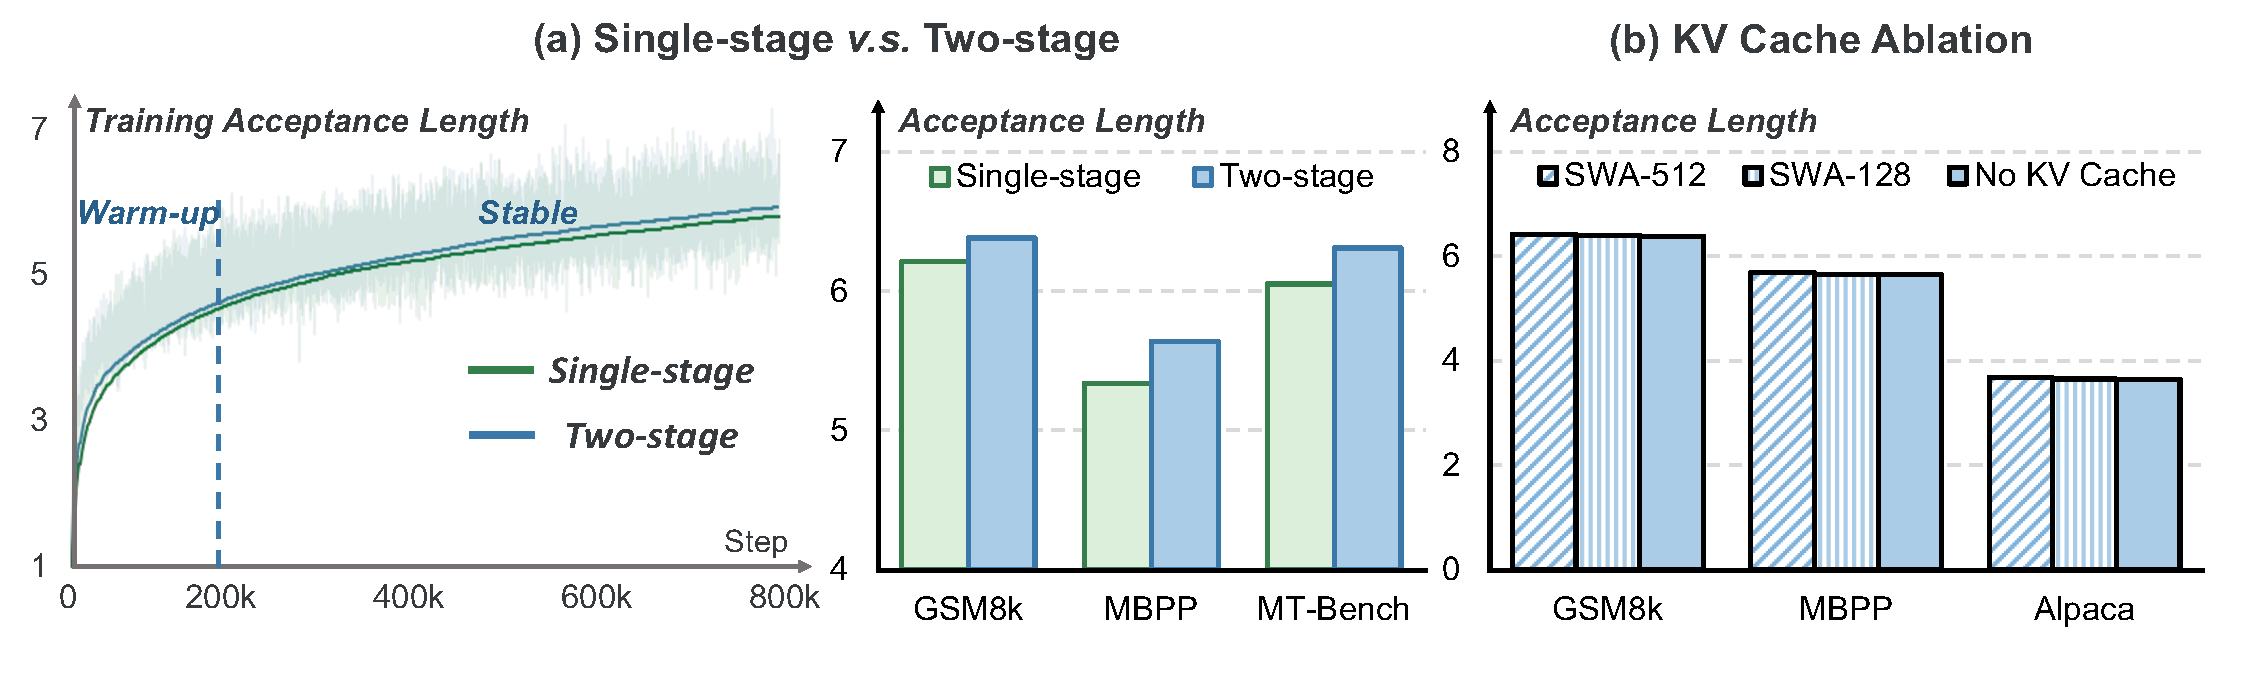
\includegraphics[width=\linewidth]{fig/ablation.pdf}
    \vspace{-20pt}
    \caption{Ablation on training strategy and KV cache.}
    \label{fig:ablation}
    % \vspace{-10pt}
\end{figure}

\textbf{Training strategy.}  Figure~\ref{fig:ablation}(a) compares our two-stage training strategy with direct single-stage training. The two-stage strategy consistently achieves higher acceptance length throughout the stable stage and improves the final performance. This result supports our motivation in Section~\ref{sec:DLite:train}: the history-aware isomorphic teacher provides an effective optimization bridge before direct alignment.

\textbf{Historical KV cache.} To examine whether historical draft states are necessary for accurate speculation, we additionally train two variants with sliding-window KV caches of 128 and 512 tokens using the same training data and setup as \we. As shown in Figure~\ref{fig:ablation}(b), after sufficient training, the three models achieve comparable acceptance lengths across the evaluated benchmarks. This suggests that historical KV states can facilitate prediction at earlier stages of training, but their advantage diminishes as the drafter learns to exploit contextual information transferred through the target hidden states. With sufficient training, \we can therefore achieve comparable quality without explicitly maintaining KV cache.



\textbf{Design space exploration.} We further explore several architectural design choices of \we, including the number of hidden states extracted from the target model, how multiple target hidden states are composed (feature-wise versus sequence-wise concatenation), and the rank of the lightweight sequential head. These dimensions jointly determine the trade-off between contextual representation capacity, drafting quality, and execution overhead. We use this design-space exploration in Appendix~\ref{app:dse} to determine the final configurations reported in Section~\ref{sec:exp:setup}.